\section{Histogram and Boxplot}
\subsection{Histogram}
In this section the histograms of the attributes will be covered. In the next section the boxplots for the attributes are explained. The attributes will be explained in details there.
\begin{figure}[H]
\centering
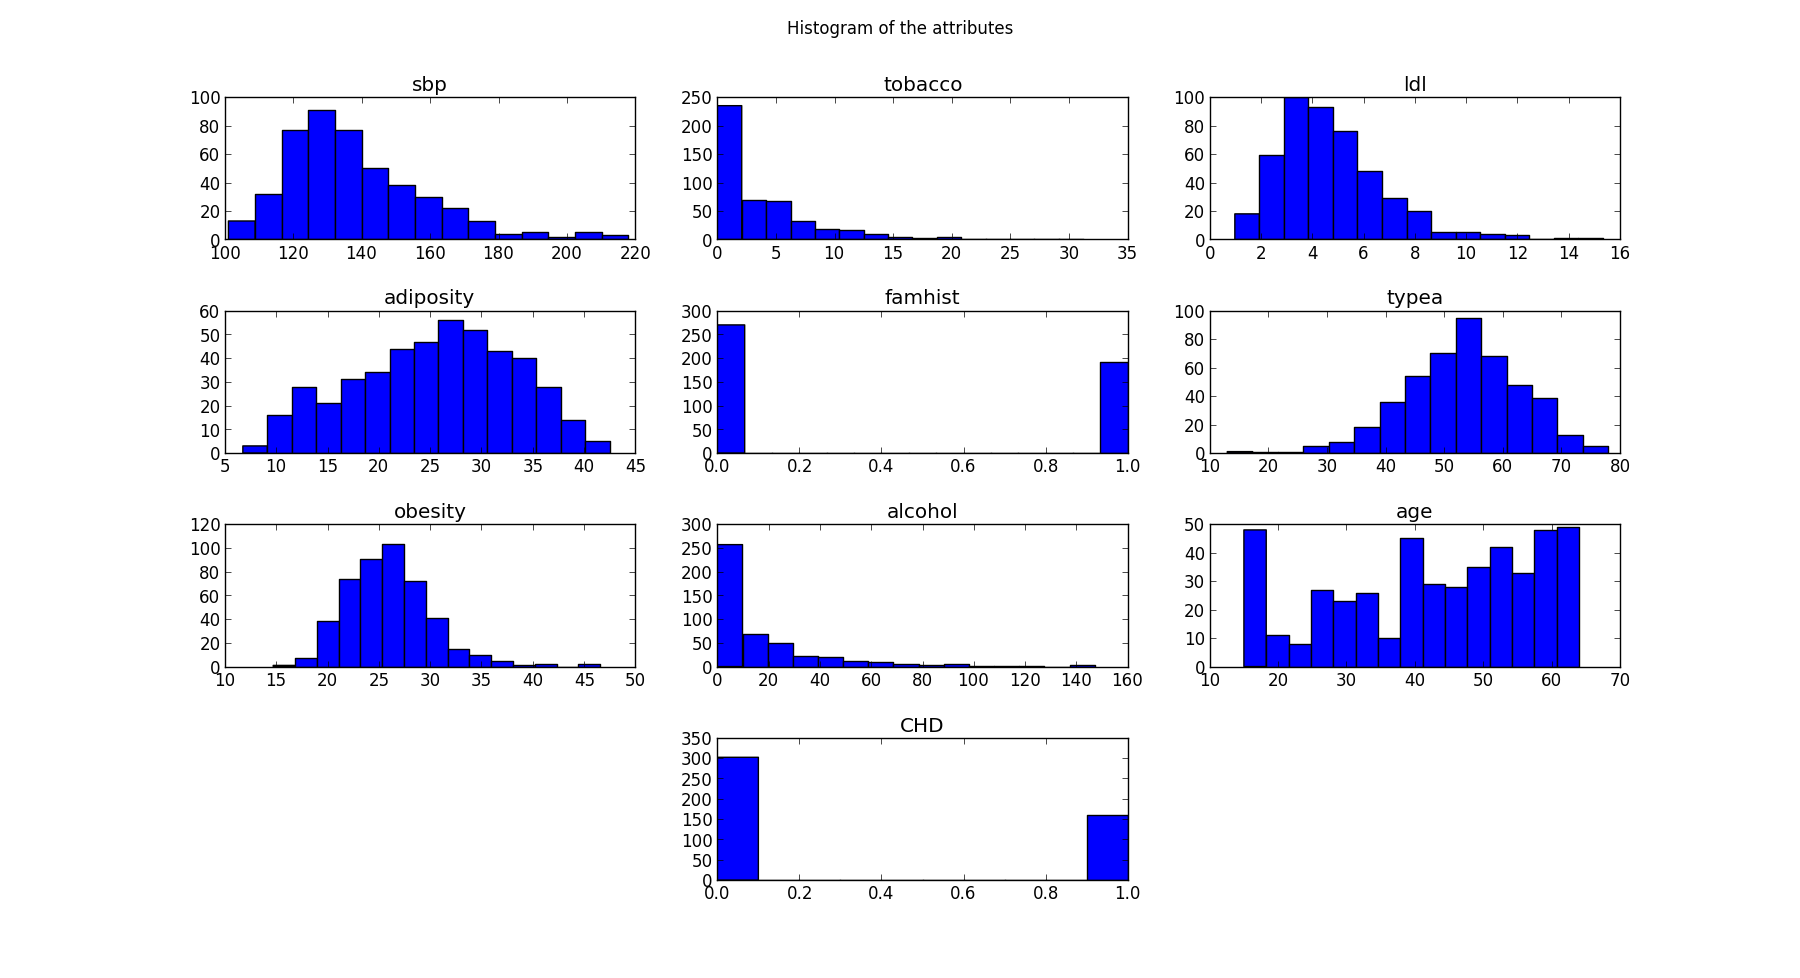
\includegraphics[width=11cm, keepaspectratio=true]{pictures/histogram.png}
\vspace{-0.2cm}
\caption{\footnotesize Histograms}
\vspace{-0.5cm}
\label{histogram}
\end{figure}
Several of our attributes seem to be close to normally distributed. These are listed below:
\paragraph{Adiposity and Obesity} are closely connected, since they both concern the size of the body. How closely connected they are will be explained later.

\paragraph{Type A} is an index of aggresiveness and stresslevel of the person. This is very normally distributed, and peaks at around 55.

\paragraph{SBP - Systolic Blood Pressure} 	seems to be peaking at around 130, which is considered a little bit high, but since the SBP is rising as you get older, and the average age of our dataset is over 40, this seems reasonable. The curve is extending far to the right, which will be covered in section \ref{boxplotSection} about boxplots.

Those attributes not distributed normally are listed below:
\paragraph{Tobacco} indicates that most persons in the dataset does not smoke.
\paragraph{Famhist} Is a binary attribute. Showing a few more people in the dataset does not have any family members with CHD, than who does have family history with CHD.
\paragraph{Alcohol} looks a lot like tobacco. How closely related they are will be considered later.
\paragraph{Age} is ranging from 15 to 65, and shows there are more data from people older than 40.
\paragraph{CHD} is quite important, because this shows us that there are around 300 cases of people \textit{not} having the CHD disease, while only 160 \textit{does} have the disease. This does have an influence in the scatterplots explained later.

\subsection{Statistics of the attributes}

Below in Figure \ref{statistics}, one can see the statistics of the attributes.

\begin{figure}[H]
%\section{Statistics of attribute data}

\begin{tabular}{| l | l | l | l | l |}
\hline
 & Mean & Variance & Max & Min \\ \hline
sbp	& 138.33 & 420.10 & 218.0 & 101.0 \\ \hline
tobacco	& 3.64 & 21.10 & 31.20 & 0.0 \\ \hline
ldl	&  4.74 & 4.29 & 15.33 & 0.98 \\ \hline
adiposity & 25.41 & 60.54 & 42.49 & 6.74 \\ \hline
famhist & 0.42 & 0.24 & 1.0 & 0.0 \\ \hline
typea	& 53.10 & 96.38 & 78.0 & 13.0 \\ \hline
obesity & 26.04 & 17.76 & 46.58 & 14.70 \\ \hline
alcohol	& 17.04 & 599.32 & 147.19 & 0.0 \\ \hline
age	& 42.82 & 213.42 & 64.0 & 15.0 \\ \hline
\end{tabular}

\caption{Showing the mean, variance, maximum and minimum for the attributes.}
\label{statistics}
\end{figure}